\documentclass[12pt,a4paper]{article}
\usepackage[]{minted}
\usepackage[brazil]{babel}
\usepackage[utf8]{inputenc}
\usepackage{graphicx}
\graphicspath{{./img/}}
\usepackage{amsmath}
\usepackage{float}

\title{Relatório das Práticas 4 e 5}
\author{Vítor Barbosa}
\date{\today}

\begin{document}
\maketitle
\section{Introdução}
Nesta prática, implementaremos um cadastro de Aluno e Professor, que herdarão da classe Pessoa. Inicialmente, faremos a leitura de dados pelo console e posteriormente criaremos um novo programa com uma janela de cadastro. Este foi o conteúdo abordado na aula 4.

Conforme solicitado na aula 5, estenderemos o programa de cadastro usando uma estrutura de dados para receber e armazenar os dados cadastrados.Também exibiremos os dados. 

\section{Cadastro com o Console}
O primeiro programa é de linha de comando e conta com as classes Pessoa, Aluno, Professor e o \emph{main.cpp}.

Tendo em mente que um bom código deve ser tão inteligível e bem comentado quanto possível, as explicações estão embutidas no próprio código.
\subsection*{Classe Pessoa}
\subsubsection*{pessoa.h}
\begin{minted}[frame=lines]{cpp}
#ifndef PESSOA_H
#define PESSOA_H
#include<string>

enum Tipo{GERAL,ALUNO,PROF};

class Pessoa{
protected:
std::string nome;
int idade;
Tipo tipo;

public:
Pessoa (std::string nome, int idade, Tipo tipo);
void definirNome(std::string nome);
std::string retornarNome();
void definirIdade(int idade);
int retornarIdade();
//Adicionei o Tipo para definir se é aluno ou prof ou qualquer outra coisa
Tipo retornarTipo();
virtual std::string retornarCurso();
virtual std::string retornarFormacao();
};
#endif
\end{minted}
\subsubsection*{pessoa.cpp}
\begin{minted}[frame=lines]{cpp}
#include<string>
#include "pessoa.h"

Pessoa::Pessoa (std::string nome, int idade,Tipo tipo):nome(nome),
                idade(idade),tipo(tipo){}

void Pessoa::definirNome(std::string nome){
this->nome = nome;
}

std::string Pessoa::retornarNome(){
return this->nome;
}

void Pessoa::definirIdade(int idade){
//Lançar exceção se a idade for negativa
if(idade<0) throw "Idade negativa";
this->idade = idade;
}

int  Pessoa::retornarIdade(){
return this->idade;
}

Tipo Pessoa::retornarTipo(){
return this->tipo;
}
/**
**Provi a implementação básica do método para que o compilador não acuse erro 
ao tentarmos fazer uma chamada polimórfica.Como o método é virtual, o 
compilador chamará a versão da subclasse se ele for sobreescrito.
**Por exemplo, para que possamos fazer o seguinte:
Pessoa p = new Aluno();
p.retornarCurso();
**Sem a implementação aqui, isso geraria um erro de método puramente virtual.
*/
std::string Pessoa::retornarCurso(){return "";};
std::string Pessoa::retornarFormacao(){return "";};
\end{minted}
\subsection*{Classe Aluno}
\subsubsection*{aluno.h}
\begin{minted}[frame=lines]{cpp}
#ifndef ALUNO_H
#define ALUNO_H
#include <string>
#include "pessoa.h"

class Aluno: public Pessoa{
	
private:
std::string curso;
	
public:
Aluno(std::string nome, int idade, std::string curso);
Aluno(std::string nome, int idade);
void        definirCurso(std::string curso);
//O especificador override é opcional
std::string retornarCurso() override;
};
#endif
\end{minted}
\subsubsection*{aluno.cpp}
\begin{minted}[frame=lines]{cpp}
#include "aluno.h"

//Este construtor inicializa a superclasse e a subclasse 
//usando uma lista de inicialização
Aluno::Aluno(std::string nome, int idade, std::string curso):
            Pessoa(nome, idade,ALUNO),curso(curso){}
Aluno::Aluno(std::string nome, int idade):Pessoa(nome,idade,ALUNO){}

void Aluno::definirCurso(std::string curso){
this->curso = curso;
}
std::string Aluno::retornarCurso() {
return this->curso;
}
\end{minted}
\subsection*{Classe Professor}
\subsubsection*{professor.h}
\begin{minted}[frame=lines]{cpp}
#ifndef PROFESSOR_H
#define PROFESSOR_H
#include "pessoa.h"

class Professor: public Pessoa{

private:
std::string formacao;

public:
Professor(std::string nome, int idade, std::string formacao);
Professor(std::string nome, int idade);
void        definirFormacao(std::string);
std::string retornarFormacao() override;
};
#endif
\end{minted}

\subsubsection*{professor.cpp}

\begin{minted}[frame=lines]{cpp}
#include "professor.h"

//Construtores com lista de inicialização
Professor::Professor(std::string nome, int idade, std::string formacao):
                    Pessoa(nome,idade,PROF),formacao(formacao){}
Professor::Professor(std::string nome, int idade):Pessoa(nome,idade,PROF){}
void        Professor::definirFormacao(std::string formacao){
this->formacao = formacao;
}
std::string Professor::retornarFormacao(){
return this->formacao;
}
\end{minted}

\subsection*{Arquivo main.cpp}
\begin{minted}[frame=lines]{cpp}
/*
Compile com g++ main.cpp aluno.cpp pessoa.cpp professor.cpp* -o main.exe
Ou simplesmente: g++ *.cpp -o main.exe
*/
#include <iostream>
//Para usar a função toupper() do C
#include <ctype.h>
#include "pessoa.h"
#include "aluno.h"
#include "professor.h"
#include <typeinfo>

//O std::vector permite acesso aleatório. 
//A std::list não, mas tem inserção e remoção em tempo constante
//O std::array é como o vector, mas tem tamanho fixo

#include<vector>

using namespace std;

int main (int argc, char **argv){

/*É obrigatório que o vetor armazene os ponteiros 
* Em c++, se você armazenar uma cópia da subclasse numa variável do tipo 
 superclasse, ocorre o problema de slicing.Ele consiste na perda das
 partes da subclasse, só o que é da super é armazenado. 
*A solução é armazenarmos os ponteiros para a subclasse na variável do 
 tipo da superclasse
*/
    vector<Pessoa*> pessoas;
    char opt;

    while(true){
        //Comandos para limpar o stdin. Sem eles, pode ficar algum caractere
        //no buffer e as instruções serão impressas várias vezes
        cin.clear();
        fflush(stdin);

        cout<<"\nOla! Selecione uma opcao: \n";
        cout<<"A- Adicione aluno, P- Adicione professor,\
               L- listar, S- Sair \n";
        cout<<"Ha "<<pessoas.size()<<" entradas\n";
        string nome;
        string extra;
        string opt_line;
        int idade ;
        getline(cin,opt_line);
        opt = opt_line[0];
        opt = toupper(opt);
        if(opt=='A'||opt=='P'){
            string s;
            cout<<"Digite o nome: \n";
            getline(cin,nome);
            cout<<"Digite a idade \n";
            getline(cin,s);
            bool except = false;
            try{idade = stoi(s);}catch(exception e){except = true;}
            if(idade<0||except) cout<<"Idade invalida \n";
            else if(opt=='A'){
                cout<<"Digite o curso: \n";
                cin>>extra;
                Aluno *a = new Aluno(nome,idade,extra);
                //cout<<a->retornarCurso();
                pessoas.push_back(a);
            }
            else{
                cout<<"Digite a formacao: \n";
                getline(cin,extra);
                Professor *prof = new Professor(nome,idade,extra);
                pessoas.push_back(prof);
            }
        }
        else if (opt=='L'){
            for(Pessoa *p :pessoas){
                cout<<"Nome: "<<p->retornarNome()<<endl;
                cout<<"Idade: "<<p->retornarIdade()<<endl;
                if(p->retornarTipo()==ALUNO){
                    cout<<"Eh um aluno."<<endl;
                    cout<<"Curso: "<<p->retornarCurso()<<endl;
                }
                else if (p->retornarTipo()==PROF){
                    cout<<"Eh um professor."<<endl;
                    cout<<"Formacao: "<<p->retornarFormacao()<<endl;
                } 
            }
        } 
        else if(opt=='S'){
            pessoas.clear();
            break;
        }
    }
    return 0;
}
\end{minted}

\section{Resultado no Console}

Vejamos uma captura de tela da execução do programa abaixo.
\begin{figure}[H]
	\centering
	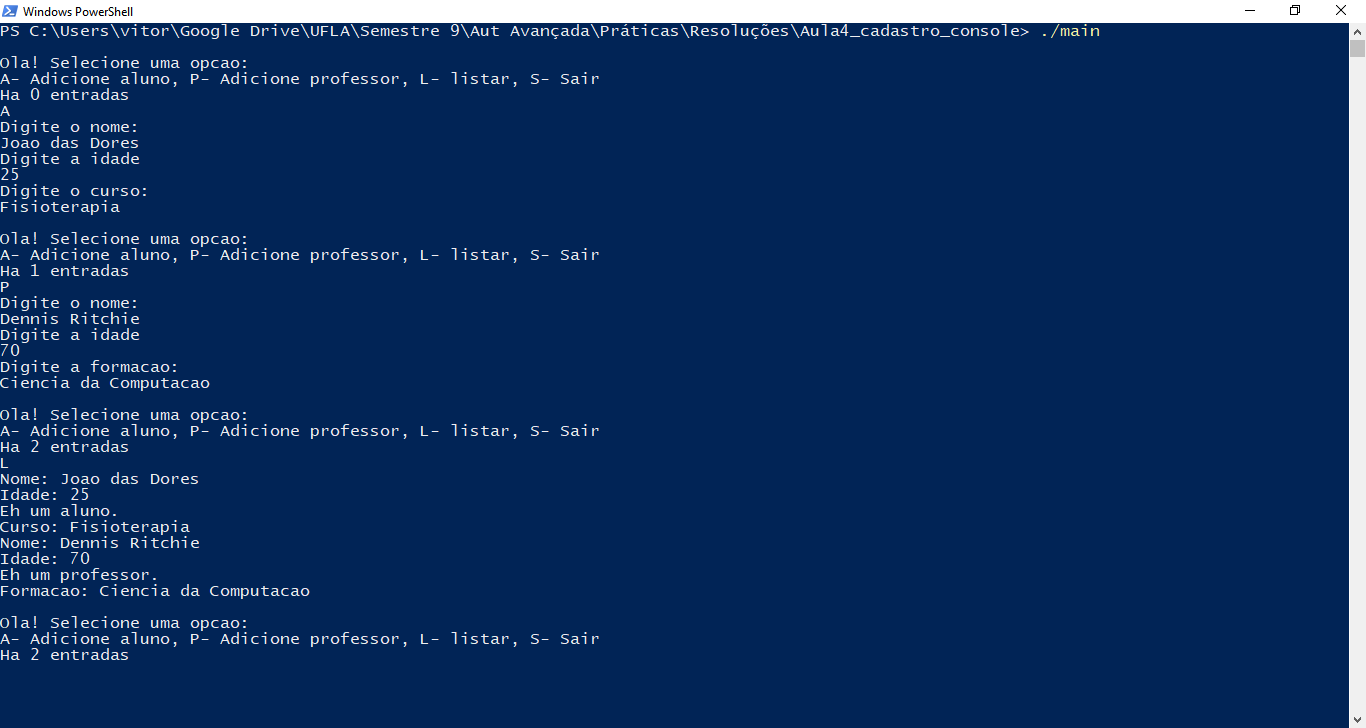
\includegraphics[width=\textwidth]{console}
	\caption{Teste da Aplicação}
\end{figure}
\section{Cadastro com Interface Gráfica}
Todos os arquivos do programa para console foram mantidos, com exceção do \emph{main.cpp}, e compuseram o que denominei \emph{libCadastro}, como pode ser visto na figura \ref{libcadastro}.
\begin{figure}[H]
\centering
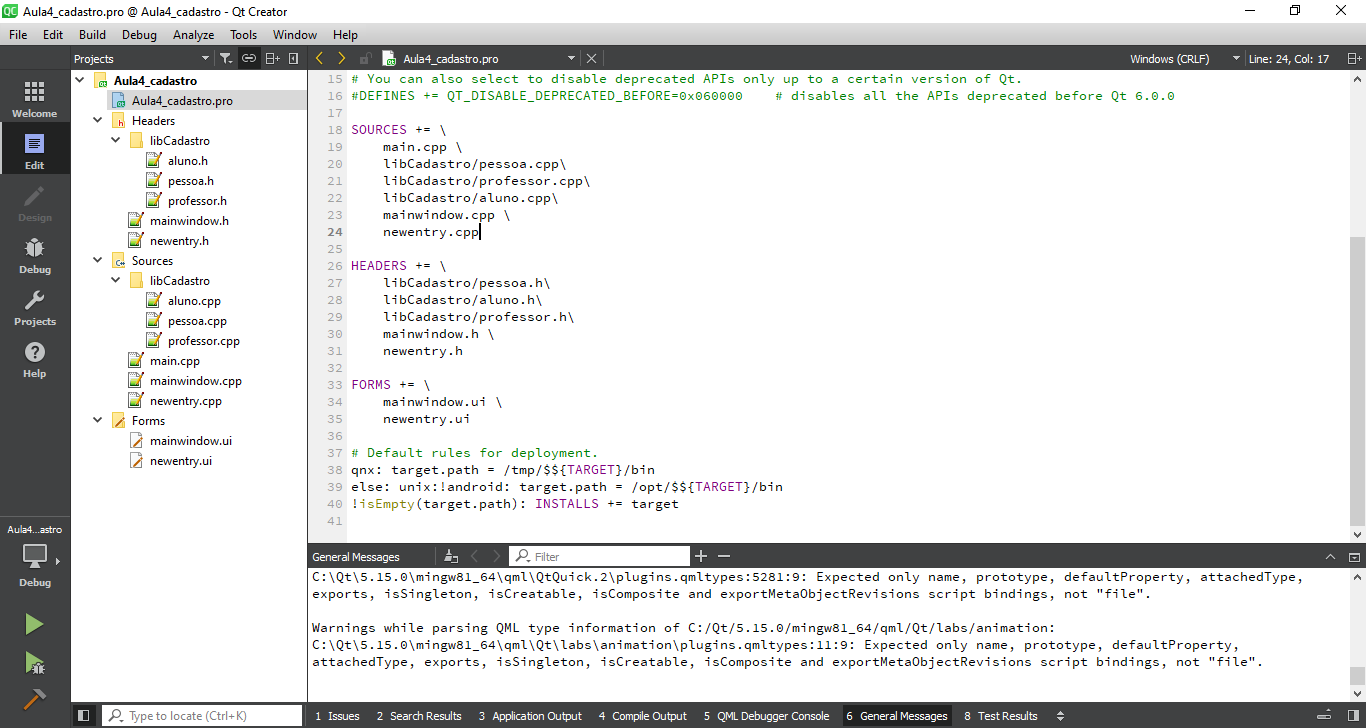
\includegraphics[width=\textwidth]{libCadastro}
\caption{Arquivo \emph{.pro} mostrando a inclusão das classes}
\label{libcadastro}
\end{figure}

\subsection*{Formulários de Cadastro e Exibição}

Os formulários de cadastro e exibição(janela principal) foram feitos graficamente no Qt Creator, como pode ser visto nas figuras \ref{mainform} e \ref{newform}.
\begin{figure}[H]
\centering
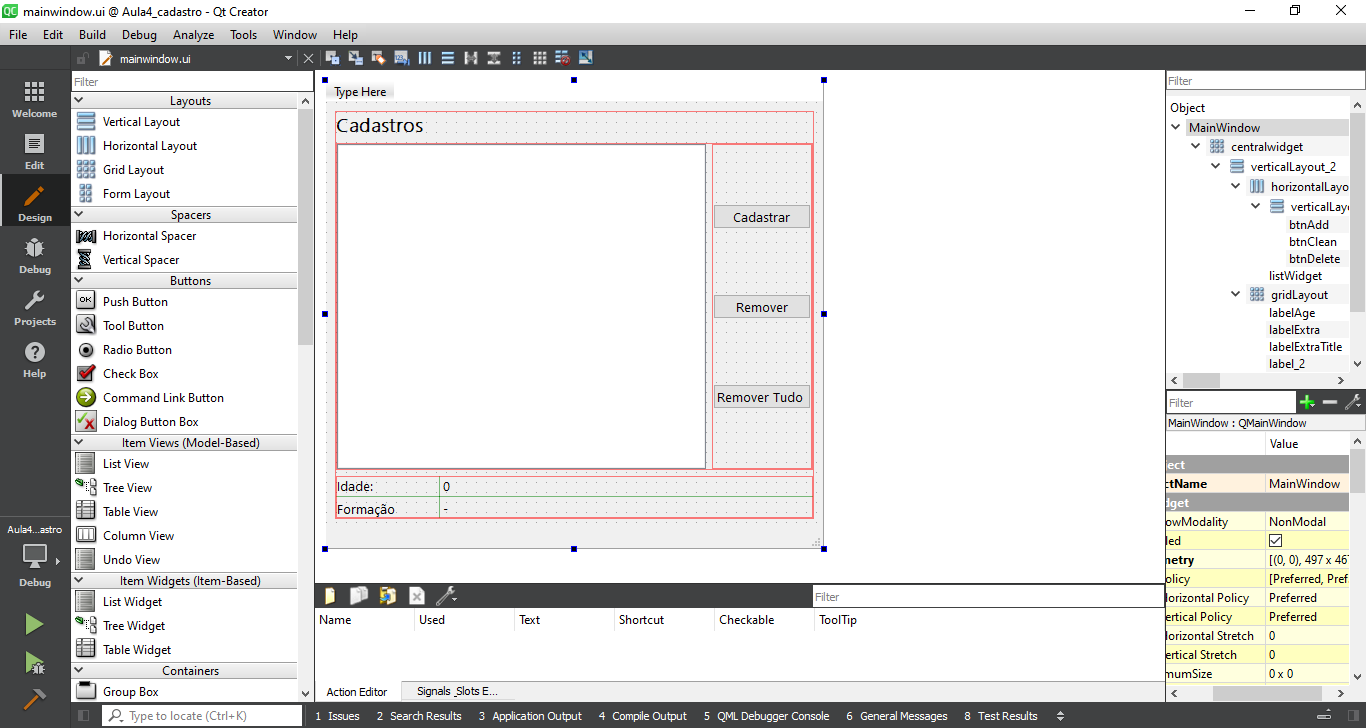
\includegraphics[width=\textwidth]{mainwin_edit}
\caption{Criação do Formulário de Exibição}
\label{mainform}
\end{figure}

\begin{figure}[H]
	\centering
	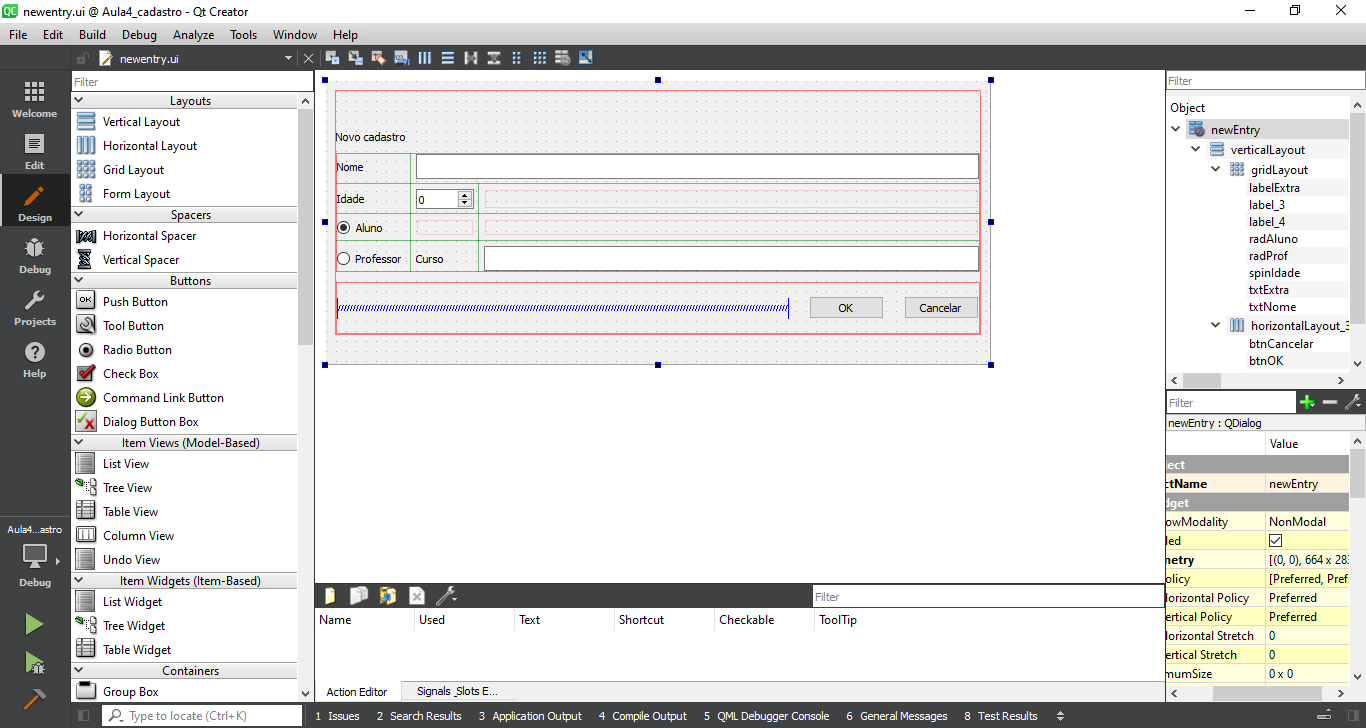
\includegraphics[width=\textwidth]{new_edit}
	\caption{Criação do Formulário de Novo Cadastro}
	\label{newform}
\end{figure}

\subsection*{mainwindow.h}

A Classe MainWindow contém a janela principal, que lista e exibe os cadastros.
Este é seu arquivo de cabeçalho.

\begin{minted}[frame=lines]{cpp}
#ifndef MAINWINDOW_H
#define MAINWINDOW_H

#include <QMainWindow>
#include "newentry.h"
#include "libCadastro/aluno.h"
#include "libCadastro/professor.h"

QT_BEGIN_NAMESPACE
namespace Ui { class MainWindow;}
QT_END_NAMESPACE

class MainWindow : public QMainWindow
{
Q_OBJECT

public:
MainWindow(QWidget *parent = nullptr);
~MainWindow();

private slots:
void on_btnAdd_clicked();
void on_btnDelete_clicked();
void on_btnClean_clicked();
void on_listWidget_currentRowChanged(int currentRow);

private:
Ui::MainWindow *ui;
newEntry *janelaCadastro;
QVector<Pessoa*> pessoas;

void updateList();
void changeEvent(QEvent *event);
};
#endif // MAINWINDOW_H
\end{minted}

\subsection*{mainwindow.cpp}

\begin{minted}[frame=lines,breaklines]{cpp}
#include "mainwindow.h"
#include "ui_mainwindow.h"
#include "newentry.h"
#include <QTextStream>

MainWindow::MainWindow(QWidget *parent): QMainWindow(parent), ui(new Ui::MainWindow){
    ui->setupUi(this);
    janelaCadastro = nullptr;
}

MainWindow::~MainWindow(){delete ui;}

void MainWindow::on_btnAdd_clicked()
{
    //Não use delete ou o programa vai dar crash, o Qt já gerencia a memória de forma transparente
    //if(janelaCadastro!=nullptr) delete janelaCadastro;

    //MUITO IMPORTANTE
    //Precisamos passar o endereço de memória do nosso vetor de pessoas, para que ele seja modificado pela outra janela
    //Use ponteiros sempre que possível, e evite variáveis referência. Ex.: use Pessoa *p em vez de Pessoa &p
    janelaCadastro = new newEntry(this,&(this->pessoas));
    janelaCadastro->show();
    this->hide();

}

void MainWindow::updateList(){
ui->listWidget->clear();
    for(Pessoa *p: pessoas){
        ui->listWidget->addItem((QString::fromStdString(p->retornarNome()))
        .prepend(p->retornarTipo()==PROF?"Professor - ":(p->retornarTipo()==ALUNO?"Aluno  ---  ":"")));
    }
}

void MainWindow::changeEvent(QEvent *e){

    QWidget::changeEvent(e);
    if(e->type()==QEvent::ActivationChange)
        if(this->isActiveWindow()){
            updateList();
        }
}

void MainWindow::on_btnDelete_clicked(){
    if(!pessoas.isEmpty())
        pessoas.pop_back(),updateList();
}

void MainWindow::on_btnClean_clicked(){
    if(!pessoas.isEmpty())
        pessoas.clear(),updateList();
}

void MainWindow::on_listWidget_currentRowChanged(int currentRow){
    //Limite o índice ou teremos um bug ao acessar o vetor
    currentRow = currentRow>(pessoas.size()-1)? 0 : (currentRow<0? 0:currentRow);

    Pessoa* p = pessoas.at(currentRow);
    ui->labelAge->setText(QString::number(pessoas.at(currentRow)->retornarIdade()));
    if(p->retornarTipo()==PROF){
        ui->labelExtraTitle->setText("Prof. Formação:  ");
        ui->labelExtra->setText(QString::fromStdString(p->retornarFormacao()));
    }
    else if(p->retornarTipo()==ALUNO){
        ui->labelExtraTitle->setText("Aluno. Curso:    ");
        ui->labelExtra->setText(QString::fromStdString(p->retornarCurso()));
    }
}
\end{minted}

\subsection*{newentry.h}
A Classe NewEntry contém as rotinas para criação de novos cadastros. Este é seu cabeçalho.
\begin{minted}[frame=lines]{cpp}
#ifndef NEWENTRY_H
#define NEWENTRY_H

#include <QDialog>
#include "libCadastro/aluno.h"
#include "libCadastro/professor.h"
#include <QMessageBox>

namespace Ui {
class newEntry;
}

class newEntry : public QDialog{
    Q_OBJECT
public:
    newEntry(QWidget *parent, QVector<Pessoa*> *pessoas);
    ~newEntry();

private slots:
    void on_btnOK_clicked();
    void on_btnCancelar_clicked();
private:
    Ui::newEntry *ui;
    QWidget *parent;
    QVector <Pessoa*> *pessoas;

    void init();
    void goBack(); //Volta à janela principal

};
#endif // NEWENTRY_H
\end{minted}

\subsection*{newentry.cpp}
\begin{minted}[frame=lines,breaklines]{cpp}
	#include "newentry.h"
#include "ui_newentry.h"
#include "container.h"

void newEntry::init(){
    QString strAluno = "Curso     ";
    QString strProf =  "Formação  ";

    QObject::connect(ui->radProf,&QRadioButton::toggled,this,[=]{
        ui->labelExtra->setText(ui->radProf->isChecked()?strProf:strAluno);});
}

// Note que pessoas precisa ser um ponteiro para um vetor de ponteiros de Pessoa
// Os ponteiros de Pessoa são para evitar o slicing (perda de dados ao passar um tipo subclasse para a superclasse
// O ponteiro para o vetor é porque desejamos modificar e repassar os dados no lugar
//Evite aramzenar referências, pois elas são confusas e causam erros
newEntry::newEntry(QWidget *parent,QVector<Pessoa*> *pessoas):QDialog(parent),
    ui(new Ui::newEntry),pessoas(pessoas){

    ui->setupUi(this);
    this->parent = parent;
   init();
   //QMessageBox::information(this,"Info","Pessoas passado");

}

newEntry::~newEntry(){ delete ui; }

void newEntry::goBack(){
    this->close();
    parent->show();
}


void newEntry::on_btnOK_clicked()
{
    bool dadosOK = true;
    QString nome = ui->txtNome->toPlainText();
    int idade = ui->spinIdade->value();
    QString extra = ui->txtExtra->toPlainText();

    // Validando os dados
    if(nome.isEmpty()) dadosOK = false;
    if(dadosOK){
        if(ui->radAluno->isChecked())
            pessoas->push_back(new Aluno(nome.toStdString(),idade,extra.toStdString()));
        else if(ui->radProf->isChecked())
            pessoas->push_back(new Professor(nome.toStdString(),idade,extra.toStdString()));
    QMessageBox::about(this,QString::fromStdString(pessoas->last()->retornarNome()),"Cadastrado com Sucesso!");
    }
    else QMessageBox::warning(this,"Erro","O nome não pode estar em branco");

    if(dadosOK){
        goBack();
    }
}

void newEntry::on_btnCancelar_clicked(){ goBack(); }
\end{minted}

\subsection*{main.cpp}
Código padrão gerado pelo Qt creator, igual ao da prática anterior e não será incluído aqui.

\section{Execução do Programa com Interface Gráfica}
O programa com janelas funcionou como esperado e alguns testes podem ser vistos a seguir.
\begin{figure}[H]
    \centering
    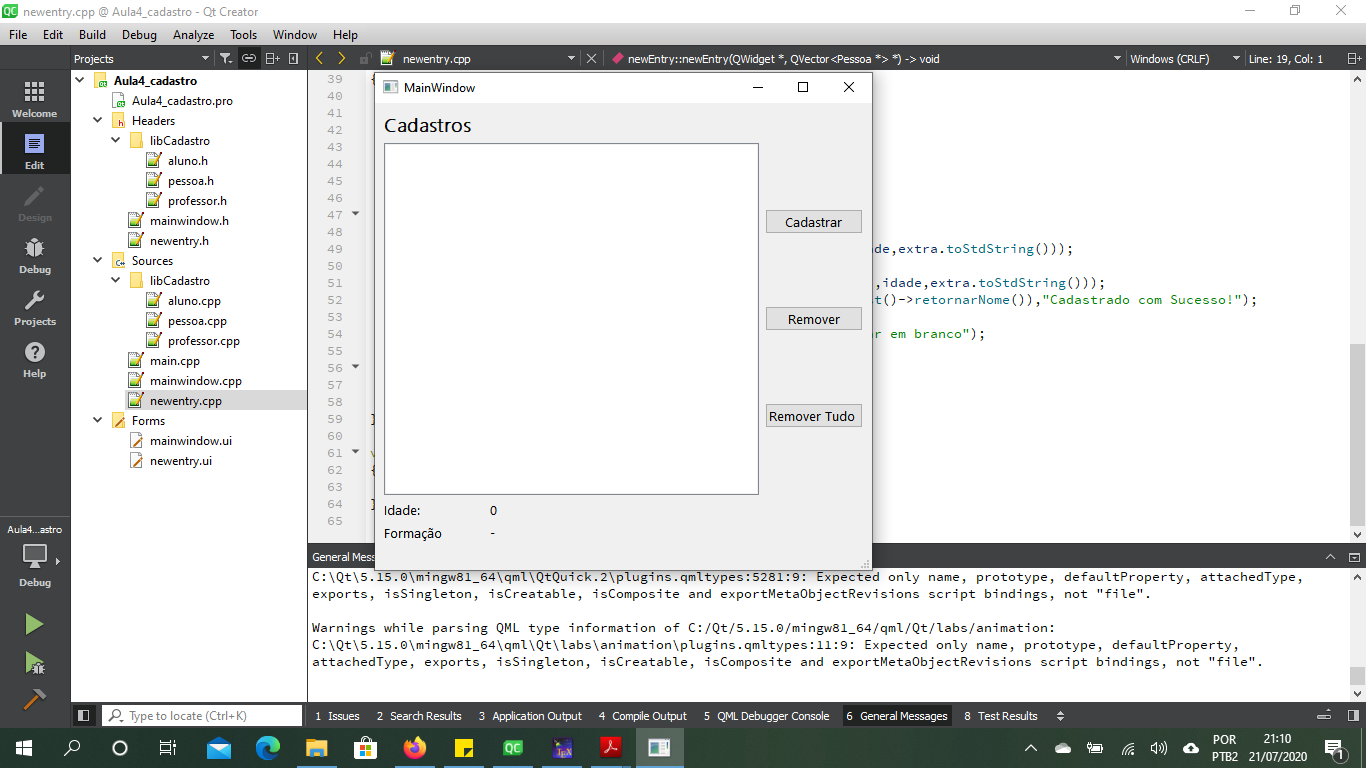
\includegraphics[width=\textwidth]{teste_vazio}
    \caption{A Janela Principal logo após o início do programa}
    \label{teste_empty}
\end{figure}
As figuras \ref{new_aluno} e \ref{new_prof} mostram o cadastro de um aluno e um professor, respectivamente.
\begin{figure}[h]
    \centering
    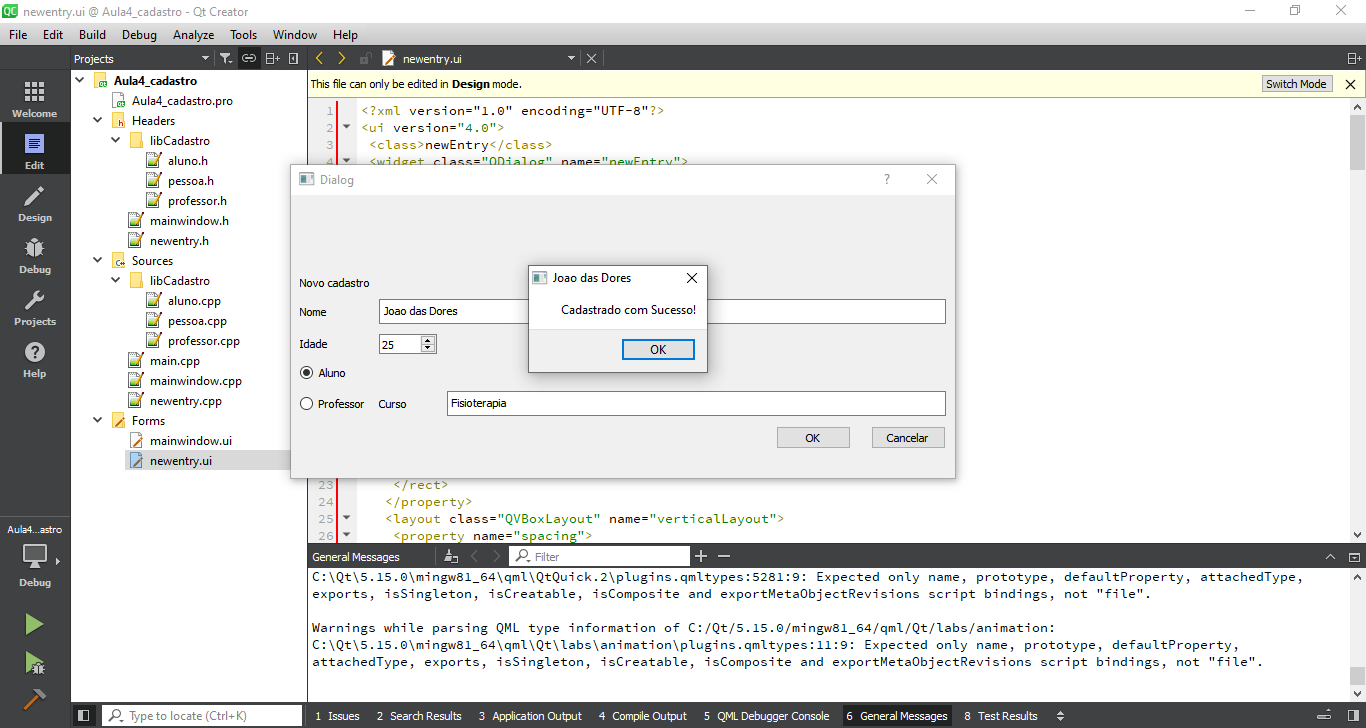
\includegraphics[width=\textwidth]{new_aluno}
    \caption{Cadastro de um Aluno}
    \label{new_aluno}
\end{figure}
\begin{figure}[h]
    \centering
    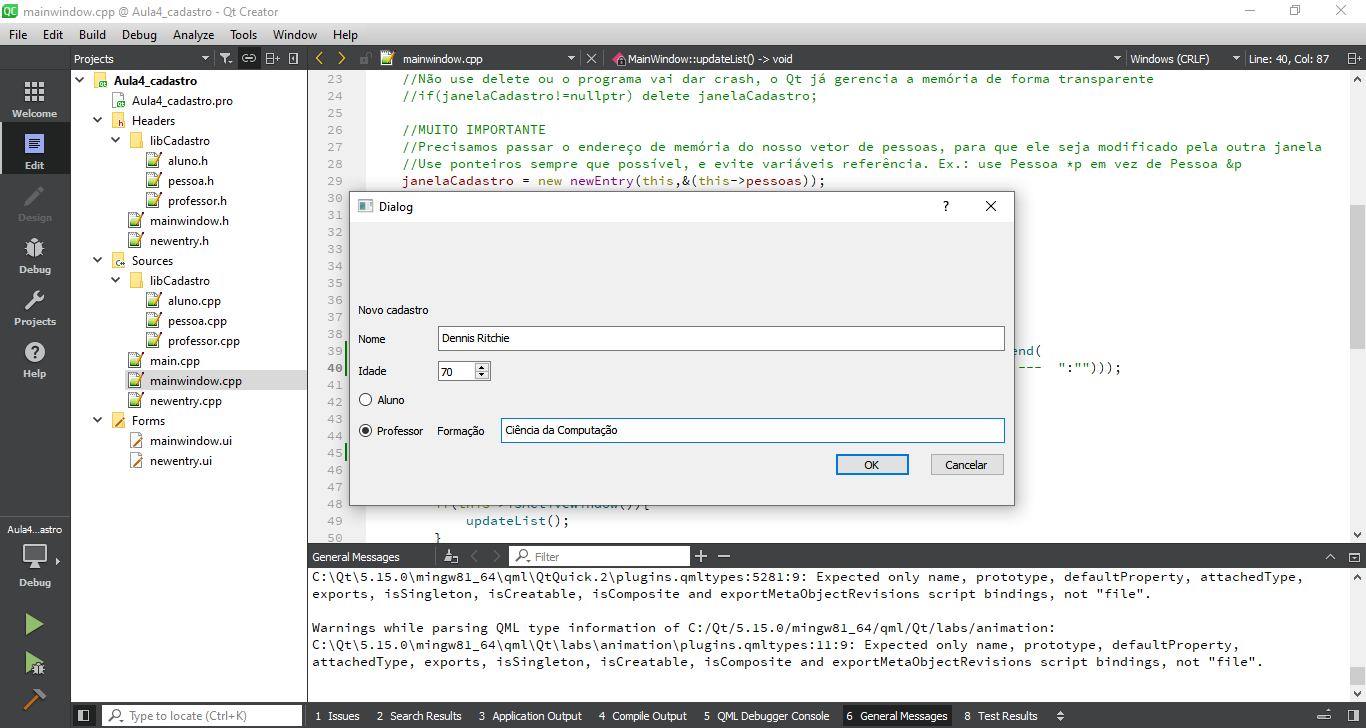
\includegraphics[width=\textwidth]{new_prof}
    \caption{Cadastro de um Professor}
    \label{new_prof}
\end{figure}

As figuras \ref{teste_aluno} e \ref{teste_prof} mostram a listagem de todos os cadastros e a exibição dos detalhes de 
um aluno e um professor, respectivamente.

\begin{figure}[h]
    \centering
    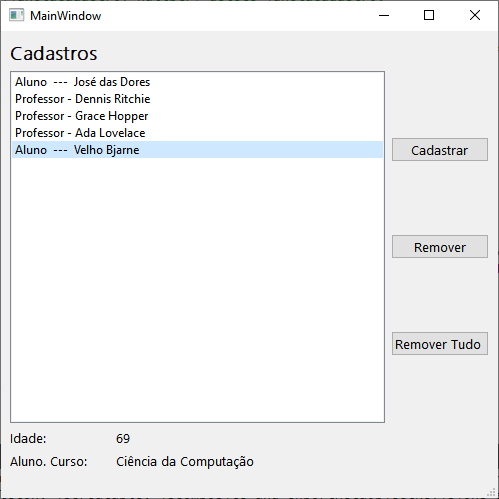
\includegraphics[width=\textwidth]{teste_aluno}
    \caption{Listagem e exibição de um Aluno}
    \label{teste_aluno}
\end{figure}
\begin{figure}[h]
    \centering
    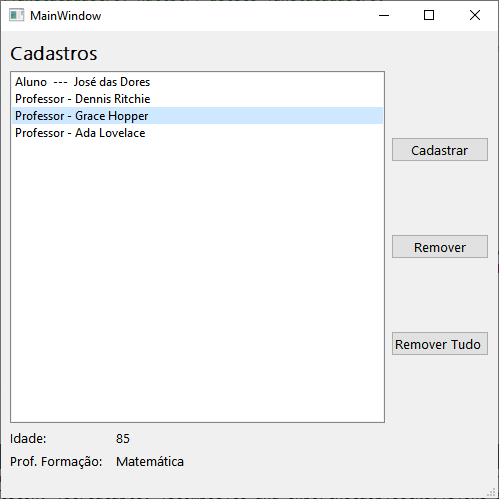
\includegraphics[width=\textwidth]{teste_prof}
    \caption{Listagem e exibição de um Professor}
    \label{teste_prof}
\end{figure}
\end{document}
